\section{Operating System Considerations}
\label{os-considerations}

Tanenbaum's \emph{Modern Operating Systems} asserts, ``The main property which
distinguishes embedded systems from handhelds is the certainty that no untrusted
software will ever run on it''~\cite{tanenbaum}. This was once true, but is no
longer the case. The Pebble~\cite{pebble} watch, for example, allows users to
load multiple third-party applications dynamically.
Embedded systems have traditionally been categorized by event-driven computation,
miniscule sleep currents, and constrained battery life. Existing embedded operating systems
have provided support for these properties and constraints. Providing support for concurrent, isolated
applications, as traditional operating systems do, provides a different set
of goals and challenges.
% %On the other hand,
% Applications for embedded systems
% are categorized by their
% % have not become more like their
% % general-purpose counterparts. Specifically, applications are still primarily
% event-driven nature with short bursts of computation rather than long-running or
% user-interactive. Moreover, embedded sleep currents and battery capacity have not
% improved significantly over the past decade.
% % so next-generation embedded systems
% % are still concerned with minimizing power consumption. 
% As a result, embedded
% systems are evolving to have requirements decendent from both previous embedded
% systems and general-purpose systems.
% The juxtaposition of these requirements
% carves a unique design space in operating systems research.
Juxtaposing these requirements and constraints drives the design considerations
for new embedded operating system design.


% They do not provide a mechanism for granting applications arbitrary direct
% hardware access for performance or peripheral requirements purposes.
%
% Note: We won't either; they'll have to implement a platform or device driver
% to access hardware directly. This is somewhat analogous to kernel modules,
% which Linux provides, albeit that kernel modules are unsafe.

% In the first evolutionary cycle of embedded devices, applications were written
% as an integral part of the runtime environment on the device. The second
% cycle brought operating systems like TinyOS~\cite{tinyos}, Contiki~\cite{contiki}, FreeRTOS~\cite{freertos} and conceptually
% separated application and OS code. Development
% % became easier allowing
% % complexity of applications to remain manageable as they grew.
% simplified,
% but the resulting
% code still compiled to a monolithic image uploaded to the device.

% Now the third evolutionary cycle is emerging: multiple and independently
% developed applications co-existing on the same device (Pebble~\cite{pebble} watch),
% and modular embedded devices
% % are becoming modular. The latter is evident with
% % multi-billion companies like Samsung, Telefonica and GE innovating with
% (SimBand~\cite{simband}, Wzzard~\cite{wzzard}, ThinkingThings~\cite{thinkingthings}, and Spotter UNIQ~\cite{spotteruniq}).
% %~\endnote{http://www.samsung.com/us/globalinnovation/innovation_areas/}, Wzzard
% %~\endnote{http://bb-smartsensing.com/wzzard-sensing-platform/}, ThinkingThings
% %~\endnote{http://www.thinkingthings.telefonica.com/}, Spotter UNIQ
% %~\endnote{https://www.quirky.com/shop/982-spotter-uniq-customizable-multipurpose-sensor}
% % The aim is to create a core hardware platform where adding sensory
% % peripherals is done by the consumer in a Lego-like fashion while the developer compiles the
% % application with the provided SDK.
% %this paragraph needs rephrasing

% These trends completely change the way applications for the embedded devices
% have been developed over the last five decades. Developers have very little control over the
% application execution model, its coexistence with other application, and which
% peripherals are connected to the embedded device. Instead application developers
% expect that the underlying operating system will perform fair resource allocation,
% protecting the application from malicious or malfunctioning applications and
% peripherals.

\subsection{General-Purpose Requirements}

In traditional embedded systems, application code is completely trusted with
full access to all hardware resources.
Applications written and controlled by a single developer make this reasonable.
% This is reasonable because applications
% were not written by third-parties and were typically not updated by end-users.
However, new embedded devices, like Pebble,
allow third-party applications and the end-user to dynamically load
applications from an app store.
A modern operating system for embedded devices must support loading applications
dynamically by the end-user. It must also protect the hardware and
kernel from these applications and applications from one another.
Modern general-purpose operating systems use hardware features such as
virtual memory and hardware virtualization to isolate applications. While these
features are not available in embedded microcontrollers, embedded operating
systems must use the tools at their disposal to achieve similar goals.

\subsection{Embedded Requirements}
\label{sec:os:execution}

Porting general-purpose operating systems, like Linux, to microcontrollers is
not the answer First, embedded systems today are still bound by power
consumption requirements. Many such embedded devices are battery powered and,
while microcontrollers have become more featureful, they do not consume less
power than previous generations.  Second, embedded applications are
significantly different than applications on general-purpose systems. Embedded
applications are event-driven, responding to timers, packet arrival, sensor
interrupts, etc., with short bursts of computation. General-purpose
applications, on the other hand, typically use
threaded execution, which may include long-running computations or latency
sensitive user interactions. Even where general-purpose systems support
event-driven programming models has largely focused on
latency, throughput and scalability~\cite{epoll,libasync,ninja} rather than
power consumption, which is typically more important in embedded devices.
Finally, embedded applications often require direct access to underlying
hardware resources. Some general-purpose operating systems have attempted to
make dynamically loaded more safe using lightweight hardware protection
domains~\cite{nooks}. However, we argue that in embedded systems,
\emph{applications} should have direct access to hardware resources when those
resources are not shared or the hardware can do isolation by
itself~\cite{ix:osdi2014}.

% %% not sure if this figure is needed
% % \begin{figure}
% %  \centering
% % 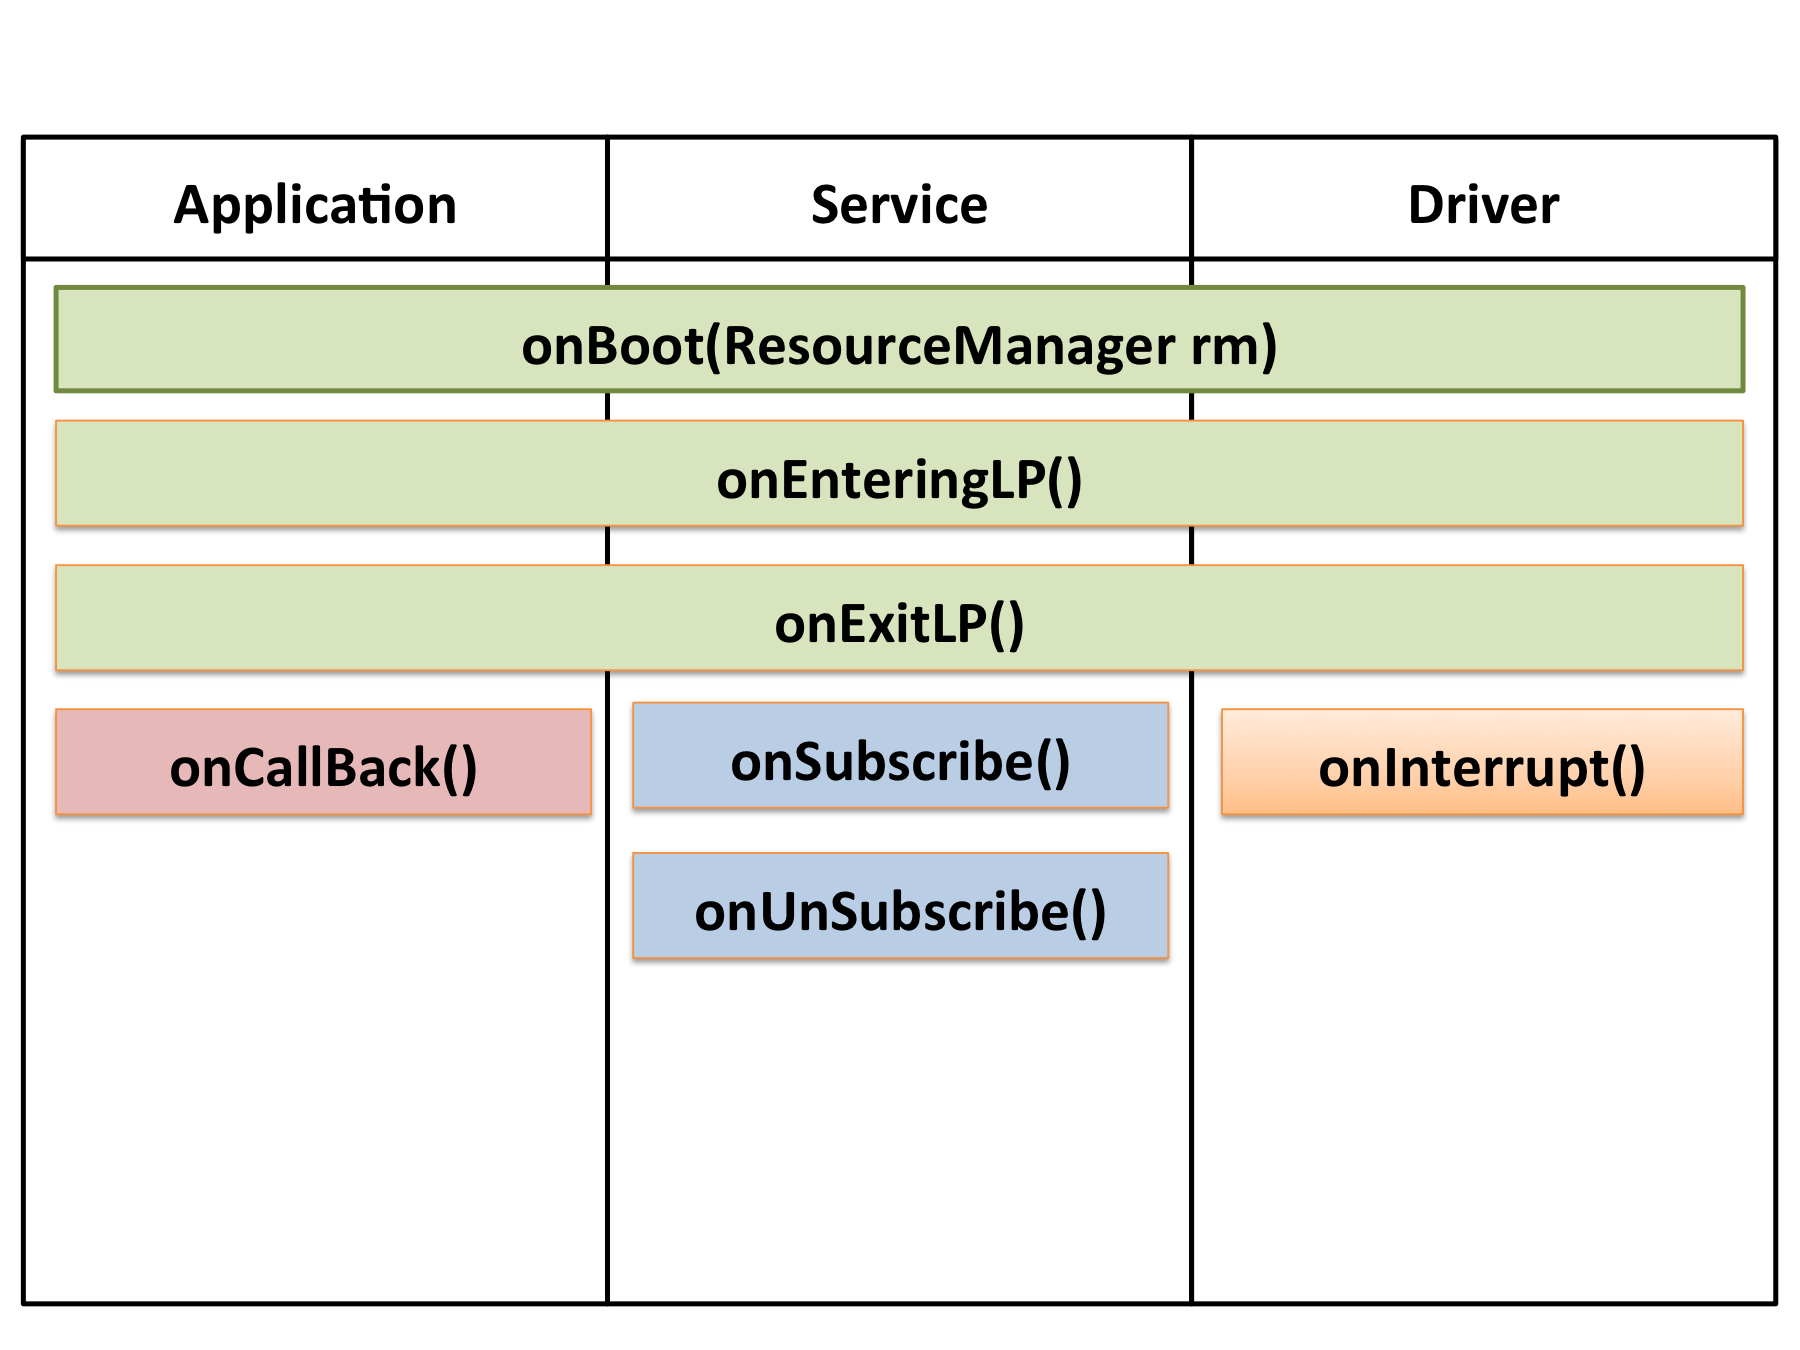
\includegraphics[width=1\columnwidth]{img/appcycle.png}
% % \caption{Runnable life cycle.}
% %  \label{fig:appcycle}
% % \end{figure}
% It's is not sufficient for a modern operating system allowing multiple
% simultaneous applications only have an event driven or preemptive
% multi-threading. In traditional OS the applications are not interrupted for
% longer period of times and in most of the cases there is no competition for
% resources. Resources need to be fairly distributed and applications, services or
% drivers notified upon event that effects program flow. Critical events are
% initialization of the application, the device is going to or waking up from low
% power mode as well secondary event like interrupts, timer, radio etc.
% % left here for event-driven e.g. Sergio add

% to allow attache new
% peripherals and load they drivers, start new services, and load/unload
% applications. The OS is expected to be a full scale modern OS except it has to
% handle all of the constrain of OS for embedded devices. Unlike most desktop and
% server applications, embedded applications must continue to run without end-user
% intervention. There is no console to indicate to the user that an application
% has crashed. Even if a crash could be communicated to the user, there is little
% action they could take. While a Blue-Screen-Of-Death is annoying on a desktop or
% server, it is unacceptable in embedded systems. Moreover, given the variety of
% devices, the OS should allow developer to use any language supporting
% Application Binary Interface, ABI.

% With resource sharing between applications and the end of exclusively trusted
% software on embedded devices comes the need for better protection guarantees
% from the operating system. The operating system must arbitrate and moderate
% access to hardware resources and protect kernel memory from misbehaving
% applications.  Further, embedded applications must continue to run without
% end-user intervention as there is often little recourse for users to detect
% and correct system error.


% % isolation incoming somewere here
% Besides separating drivers for core peripherals (SPI, USART, GPIO, etc) and
% device drivers (radio, flash, etc) into separate layers. Modern OS has to
% enforce safety policies not only on applications but also on device drivers. The
% OS has to ensure that at most one driver has access to a specific hardware
%  resource---multiplexing must be done explicitly in the core peripheral driver
%  or through an intermediate interface. Finally, the OS need to ensure that
%  device drivers cannot corrupt kernel memory or perform denial of service
%  attacks by drivers. Multiple application on the embedded device also requires
%  of to protect the kernel and other applications from malicious actions.

% While requirements have resemblance to those of a traditional OS, modern
% embedded OS has to fulfill them with the computational and energy constrains.

% energy efficency

% \name prevents drivers from subverting Rust's memory safety by restricting
% device drivers to a safe subset of the Rust language.~\endnote{Rust allows code
% to circumvent the type system using the \tt{unsafe} keyword. \name uses a
% compiler flag that disallows this keyword when compiling device drivers.} \name
% also ensures, at compile time, that at most one driver has access to a specific
% hardware resource---multiplexing must be done explicitly in the core peripheral
% driver or through an intermediate interface. Finally, \name ensures device
% drivers cannot corrupt kernel memory through careful choice of interfaces. \name
% ensures that \name does not protect the kernel from denial of service attacks by
% drivers. %wait what does this last sentence mean?




